%%*****************************************************************************
%% $Id: bst-prog.tex,v 0.00 2008/05/01 13:56:41 gene Exp $
%%*****************************************************************************
%% Author: Gerd Neugebauer
%%-----------------------------------------------------------------------------
\begingroup
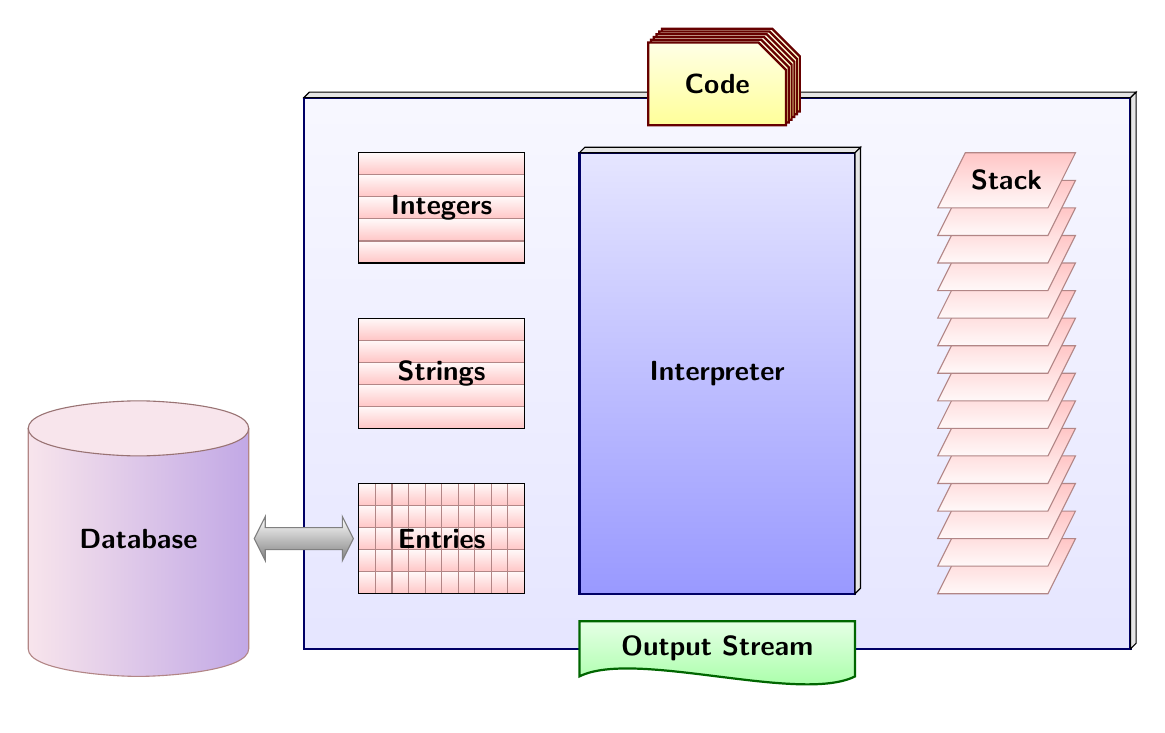
\begin{tikzpicture}[scale=.7]\sf\bfseries
  % --- bottom layer ---
  \shade[top color=white!97!blue,bottom color=white!90!blue,draw=blue!40!black,thick]
  (0,0) rectangle (15,10);
  \draw[fill=gray!20!white] (0,10) -- (.1,10.1) -- (15.1,10.1) -- (15,10) -- cycle;
  \draw[fill=gray!20!white] (15,10) -- (15.1,10.1) -- (15.1,.1) -- (15,0) -- cycle;

  % --- code ---
  \begin{scope}[shift={(6.25,9.5)},scale=.5]
    \begin{scope}[shift={(.5,.5)}]
      \shade[top color=white!90!yellow,bottom color=white!60!yellow,draw=red!40!black,thick]
      (0,0) -- (5,0) -- (5,2) -- (4,3) -- (0,3) -- cycle;
    \end{scope}
    \begin{scope}[shift={(.4,.4)}]
      \shade[top color=white!90!yellow,bottom color=white!60!yellow,draw=red!40!black,thick]
      (0,0) -- (5,0) -- (5,2) -- (4,3) -- (0,3) -- cycle;
    \end{scope}
    \begin{scope}[shift={(.3,.3)}]
      \shade[top color=white!90!yellow,bottom color=white!60!yellow,draw=red!40!black,thick]
      (0,0) -- (5,0) -- (5,2) -- (4,3) -- (0,3) -- cycle;
    \end{scope}
    \begin{scope}[shift={(.2,.2)}]
      \shade[top color=white!90!yellow,bottom color=white!60!yellow,draw=red!40!black,thick]
      (0,0) -- (5,0) -- (5,2) -- (4,3) -- (0,3) -- cycle;
    \end{scope}
    \begin{scope}[shift={(.1,.1)}]
      \shade[top color=white!90!yellow,bottom color=white!60!yellow,draw=red!40!black,thick]
      (0,0) -- (5,0) -- (5,2) -- (4,3) -- (0,3) -- cycle;
    \end{scope}
    \shade[top color=white!90!yellow,bottom color=white!60!yellow,draw=red!40!black,thick]
    (0,0) -- (5,0) -- (5,2) -- (4,3) -- (0,3) -- cycle;
  \end{scope}
  \draw (7.5,10.25) node {Code};

  % --- interpreter ---
  \shade[top color=white!90!blue,bottom color=white!60!blue,draw=blue!40!black,thick]
  (5,1) rectangle (10,9);
  \draw[fill=gray!20!white] (5,9) -- (5.1,9.1) -- (10.1,9.1) -- (10,9) -- cycle;
  \draw[fill=gray!20!white] (10,9) -- (10.1,9.1) -- (10.1,1.1) -- (10,1) -- cycle;
  \draw (7.5,5) node {Interpreter};
  
  \shade[top color=white!90!green,bottom color=white!60!green,draw=green!40!black,thick]
  (5,-.5) .. controls (6,0) and (9,-1) .. (10,-.5) -- (10,.5) -- (5,.5) -- cycle;
  \draw (7.5,0) node {Output Stream};


  % --- stack ---
  \shade[top color=white!10!pink,bottom color=white!90!pink,draw=pink!70!black,shift={(11.5,1)}] (0,0) -- (.5,1) -- (2.5,1) -- (2,0) -- cycle;
  \shade[top color=white!10!pink,bottom color=white!90!pink,draw=pink!70!black,shift={(11.5,1.5)}] (0,0) -- (.5,1) -- (2.5,1) -- (2,0) -- cycle;
  \shade[top color=white!10!pink,bottom color=white!90!pink,draw=pink!70!black,shift={(11.5,2)}] (0,0) -- (.5,1) -- (2.5,1) -- (2,0) -- cycle;
  \shade[top color=white!10!pink,bottom color=white!90!pink,draw=pink!70!black,shift={(11.5,2.5)}] (0,0) -- (.5,1) -- (2.5,1) -- (2,0) -- cycle;
  \shade[top color=white!10!pink,bottom color=white!90!pink,draw=pink!70!black,shift={(11.5,3)}] (0,0) -- (.5,1) -- (2.5,1) -- (2,0) -- cycle;
  \shade[top color=white!10!pink,bottom color=white!90!pink,draw=pink!70!black,shift={(11.5,3.5)}] (0,0) -- (.5,1) -- (2.5,1) -- (2,0) -- cycle;
  \shade[top color=white!10!pink,bottom color=white!90!pink,draw=pink!70!black,shift={(11.5,4)}] (0,0) -- (.5,1) -- (2.5,1) -- (2,0) -- cycle;
  \shade[top color=white!10!pink,bottom color=white!90!pink,draw=pink!70!black,shift={(11.5,4.5)}] (0,0) -- (.5,1) -- (2.5,1) -- (2,0) -- cycle;
  \shade[top color=white!10!pink,bottom color=white!90!pink,draw=pink!70!black,shift={(11.5,5)}] (0,0) -- (.5,1) -- (2.5,1) -- (2,0) -- cycle;
  \shade[top color=white!10!pink,bottom color=white!90!pink,draw=pink!70!black,shift={(11.5,5.5)}] (0,0) -- (.5,1) -- (2.5,1) -- (2,0) -- cycle;
  \shade[top color=white!10!pink,bottom color=white!90!pink,draw=pink!70!black,shift={(11.5,6)}] (0,0) -- (.5,1) -- (2.5,1) -- (2,0) -- cycle;
  \shade[top color=white!10!pink,bottom color=white!90!pink,draw=pink!70!black,shift={(11.5,6.5)}] (0,0) -- (.5,1) -- (2.5,1) -- (2,0) -- cycle;
  \shade[top color=white!10!pink,bottom color=white!90!pink,draw=pink!70!black,shift={(11.5,7)}] (0,0) -- (.5,1) -- (2.5,1) -- (2,0) -- cycle;
  \shade[top color=white!10!pink,bottom color=white!90!pink,draw=pink!70!black,shift={(11.5,7.5)}] (0,0) -- (.5,1) -- (2.5,1) -- (2,0) -- cycle;
  \shade[top color=white!10!pink,bottom color=white!90!pink,draw=pink!70!black,shift={(11.5,8)}] (0,0) -- (.5,1) -- (2.5,1) -- (2,0) -- cycle;
  \draw (12.75,8.5) node {Stack};

  % --- integers ---
  \shade[top color=white!90!pink,bottom color=white!10!pink,draw=pink!70!black]
  (1,7) rectangle (4,7.4);
  \shade[shift={(0,.4)},top color=white!90!pink,bottom color=white!10!pink,draw=pink!70!black]
  (1,7) rectangle (4,7.4);
  \shade[shift={(0,.8)},top color=white!90!pink,bottom color=white!10!pink,draw=pink!70!black]
  (1,7) rectangle (4,7.4);
  \shade[shift={(0,1.2)},top color=white!90!pink,bottom color=white!10!pink,draw=pink!70!black]
  (1,7) rectangle (4,7.4);
  \shade[shift={(0,1.6)},top color=white!90!pink,bottom color=white!10!pink,draw=pink!70!black]
  (1,7) rectangle (4,7.4);
  \draw (1,7) rectangle (4,9);
  \draw (2.5,8) node {Integers};

  % --- strings ---
  \shade[top color=white!90!pink,bottom color=white!10!pink,draw=pink!70!black]
  (1,4) rectangle (4,4.4);
  \shade[shift={(0,.4)},top color=white!90!pink,bottom color=white!10!pink,draw=pink!70!black]
  (1,4) rectangle (4,4.4);
  \shade[shift={(0,.8)},top color=white!90!pink,bottom color=white!10!pink,draw=pink!70!black]
  (1,4) rectangle (4,4.4);
  \shade[shift={(0,1.2)},top color=white!90!pink,bottom color=white!10!pink,draw=pink!70!black]
  (1,4) rectangle (4,4.4);
  \shade[shift={(0,1.6)},top color=white!90!pink,bottom color=white!10!pink,draw=pink!70!black]
  (1,4) rectangle (4,4.4);
  \draw (1,4) rectangle (4,6);
  \draw (2.5,5) node {Strings};

  % --- entries ---
  \shade[top color=white!90!pink,bottom color=white!10!pink,draw=pink!70!black]
  (1,1) rectangle (4,1.4);
  \shade[shift={(0,.4)},top color=white!90!pink,bottom color=white!10!pink,draw=pink!70!black]
  (1,1) rectangle (4,1.4);
  \shade[shift={(0,.8)},top color=white!90!pink,bottom color=white!10!pink,draw=pink!70!black]
  (1,1) rectangle (4,1.4);
  \shade[shift={(0,1.2)},top color=white!90!pink,bottom color=white!10!pink,draw=pink!70!black]
  (1,1) rectangle (4,1.4);
  \shade[shift={(0,1.6)},top color=white!90!pink,bottom color=white!10!pink,draw=pink!70!black]
  (1,1) rectangle (4,1.4);
  \draw[shift={(.3,0)},draw=pink!70!black] (1,1) -- (1,3);
  \draw[shift={(.6,0)},draw=pink!70!black] (1,1) -- (1,3);
  \draw[shift={(.9,0)},draw=pink!70!black] (1,1) -- (1,3);
  \draw[shift={(1.2,0)},draw=pink!70!black] (1,1) -- (1,3);
  \draw[shift={(1.5,0)},draw=pink!70!black] (1,1) -- (1,3);
  \draw[shift={(1.8,0)},draw=pink!70!black] (1,1) -- (1,3);
  \draw[shift={(2.1,0)},draw=pink!70!black] (1,1) -- (1,3);
  \draw[shift={(2.4,0)},draw=pink!70!black] (1,1) -- (1,3);
  \draw[shift={(2.7,0)},draw=pink!70!black] (1,1) -- (1,3);
  \draw (1,1) rectangle (4,3);
  \draw (2.5,2) node {Entries};

  \begin{scope}[shift={(-5,0)}]
    \shade[left color=white!96!blue!70!pink,right color=white!60!blue!60!pink,draw=pink!70!black]
    (0,0)   .. controls (0,-.4) and (1.5,-.5) ..
    (2,-.5)  .. controls (2.5,-.5) and (4,-.4) ..
    (4,0) -- (4,4) -- (0,4) -- cycle;
    \draw[shift={(0,4)},fill=white!96!blue!70!pink,draw=pink!60!black]
    (0,0)   .. controls (0,.4) and (1.5,.5) ..
    (2,.5)  .. controls (2.5,.5) and (4,.4) ..
    (4,0)   .. controls (4,-.4) and (2.5,-.5) ..
    (2,-.5) .. controls (1.5,-.5) and (0,-.4) ..
    (0,0);
  \end{scope}
  \draw (-3,2) node {Database};

%  \draw[shift={(0,-5)}]
%  (-.2,0) -- (0,.4) -- (0,.2) -- (1,.2) -- (1,.4) -- (1.2,0) --
%  (1,-.4) -- (1,-.2) -- (0,-.2) -- (0,-.4) -- cycle;

  \shade[shift={(-.7,2)}, top color=white, bottom color=gray,draw=gray]
  (-.2,0) -- (0,.4) -- (0,.2) -- (1.4,.2) -- (1.4,.4) -- (1.6,0) --
  (1.4,-.4) -- (1.4,-.2) -- (0,-.2) -- (0,-.4) -- cycle;

\end{tikzpicture}
\endgroup
\endinput
%
% Local Variables: 
% mode: latex
% TeX-master: nil
% End: 
